\chapter{Lecture 28 - Orthogonal Series Expansion}
\label{ch:lec28}
\section{Objectives}
\begin{itemize}
\item Apply separation of variables and solve PDEs that have solutions in the form of orthogonal series expansions (other than Fourier series).
\item Show examples with the heat and wave equation.
\end{itemize}
\setcounter{lstannotation}{0} %hack to try and re-set annotation counter.

For some sets of boundary conditions, the solution to the heat equation is an infinite series that is not a Fourier series.  I will argue that, apart from details regarding identifying eigenvalues, the implications of this are not large and will have little impact on how you go about computing the solution.  All of this is most easily clarified with a couple of examples.

\vspace{0.3cm}

\noindent\textbf{Example \#1:}  Consider the boundary value problem below based on the heat equation.
\begin{table}
\begin{tabular}{l l}
$\substack{\text{Governing} \\\text{Equation}}: $& $\frac{\partial u}{\partial t} = \alpha^2 \frac{\partial^2 u}{\partial x^2},  \ \ \alpha>0, \ \ 0<x<1, \ \ t>0$ \\
& \\
$\substack{\text{Boundary} \\ \text{Conditions}}: $& $u(0,t)=0, \ \ u_x(1,t) = -hu(1,t), \ \ h>0, \  t>0$\\
& \\
$\substack{\text{Initial} \\ \text{Conditions}}: $ & $u(x,0) = 1, \ \ 0<x<1 $ \\
\end{tabular}
\end{table}
\begin{marginfigure}
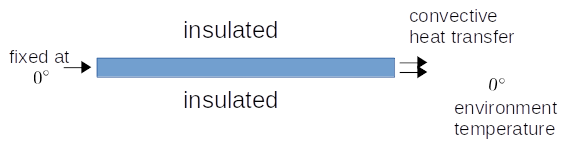
\includegraphics{lec28-ex1-schematic.png}
\caption{Schematic of Example \#1.}
\label{fig:lec28-ex1-schematic}
\end{marginfigure}
A schematic of this problem is shown in Figure \ref{fig:lec28-ex1-schematic}.  On the left end of the domain we have a type 3 boundary condition representing convective heat transfer to an environment maintained at a temperature of 0$^{\circ}$.\marginnote{Note that we have not established any physical units on this system.  If it helps, consider all temperatures given to be in degrees Celsius.}


